\documentclass[1p]{elsarticle_modified}
%\bibliographystyle{elsarticle-num}

%\usepackage[colorlinks]{hyperref}
%\usepackage{abbrmath_seonhwa} %\Abb, \Ascr, \Acal ,\Abf, \Afrak
\usepackage{amsfonts}
\usepackage{amssymb}
\usepackage{amsmath}
\usepackage{amsthm}
\usepackage{scalefnt}
\usepackage{amsbsy}
\usepackage{kotex}
\usepackage{caption}
\usepackage{subfig}
\usepackage{color}
\usepackage{graphicx}
\usepackage{xcolor} %% white, black, red, green, blue, cyan, magenta, yellow
\usepackage{float}
\usepackage{setspace}
\usepackage{hyperref}

\usepackage{tikz}
\usetikzlibrary{arrows}

\usepackage{multirow}
\usepackage{array} % fixed length table
\usepackage{hhline}

%%%%%%%%%%%%%%%%%%%%%
\makeatletter
\renewcommand*\env@matrix[1][\arraystretch]{%
	\edef\arraystretch{#1}%
	\hskip -\arraycolsep
	\let\@ifnextchar\new@ifnextchar
	\array{*\c@MaxMatrixCols c}}
\makeatother %https://tex.stackexchange.com/questions/14071/how-can-i-increase-the-line-spacing-in-a-matrix
%%%%%%%%%%%%%%%

\usepackage[normalem]{ulem}

\newcommand{\msout}[1]{\ifmmode\text{\sout{\ensuremath{#1}}}\else\sout{#1}\fi}
%SOURCE: \msout is \stkout macro in https://tex.stackexchange.com/questions/20609/strikeout-in-math-mode

\newcommand{\cancel}[1]{
	\ifmmode
	{\color{red}\msout{#1}}
	\else
	{\color{red}\sout{#1}}
	\fi
}

\newcommand{\add}[1]{
	{\color{blue}\uwave{#1}}
}

\newcommand{\replace}[2]{
	\ifmmode
	{\color{red}\msout{#1}}{\color{blue}\uwave{#2}}
	\else
	{\color{red}\sout{#1}}{\color{blue}\uwave{#2}}
	\fi
}

\newcommand{\Sol}{\mathcal{S}} %segment
\newcommand{\D}{D} %diagram
\newcommand{\A}{\mathcal{A}} %arc


%%%%%%%%%%%%%%%%%%%%%%%%%%%%%5 test

\def\sl{\operatorname{\textup{SL}}(2,\Cbb)}
\def\psl{\operatorname{\textup{PSL}}(2,\Cbb)}
\def\quan{\mkern 1mu \triangleright \mkern 1mu}

\theoremstyle{definition}
\newtheorem{thm}{Theorem}[section]
\newtheorem{prop}[thm]{Proposition}
\newtheorem{lem}[thm]{Lemma}
\newtheorem{ques}[thm]{Question}
\newtheorem{cor}[thm]{Corollary}
\newtheorem{defn}[thm]{Definition}
\newtheorem{exam}[thm]{Example}
\newtheorem{rmk}[thm]{Remark}
\newtheorem{alg}[thm]{Algorithm}

\newcommand{\I}{\sqrt{-1}}
\begin{document}

%\begin{frontmatter}
%
%\title{Boundary parabolic representations of knots up to 8 crossings}
%
%%% Group authors per affiliation:
%\author{Yunhi Cho} 
%\address{Department of Mathematics, University of Seoul, Seoul, Korea}
%\ead{yhcho@uos.ac.kr}
%
%
%\author{Seonhwa Kim} %\fnref{s_kim}}
%\address{Center for Geometry and Physics, Institute for Basic Science, Pohang, 37673, Korea}
%\ead{ryeona17@ibs.re.kr}
%
%\author{Hyuk Kim}
%\address{Department of Mathematical Sciences, Seoul National University, Seoul 08826, Korea}
%\ead{hyukkim@snu.ac.kr}
%
%\author{Seokbeom Yoon}
%\address{Department of Mathematical Sciences, Seoul National University, Seoul, 08826,  Korea}
%\ead{sbyoon15@snu.ac.kr}
%
%\begin{abstract}
%We find all boundary parabolic representation of knots up to 8 crossings.
%
%\end{abstract}
%\begin{keyword}
%    \MSC[2010] 57M25 
%\end{keyword}
%
%\end{frontmatter}

%\linenumbers
%\tableofcontents
%
\newcommand\colored[1]{\textcolor{white}{\rule[-0.35ex]{0.8em}{1.4ex}}\kern-0.8em\color{red} #1}%
%\newcommand\colored[1]{\textcolor{white}{ #1}\kern-2.17ex	\textcolor{white}{ #1}\kern-1.81ex	\textcolor{white}{ #1}\kern-2.15ex\color{red}#1	}

{\Large $\underline{12a_{1136}~(K12a_{1136})}$}

\setlength{\tabcolsep}{10pt}
\renewcommand{\arraystretch}{1.6}
\vspace{1cm}\begin{tabular}{m{100pt}>{\centering\arraybackslash}m{274pt}}
\multirow{5}{120pt}{
	\centering
	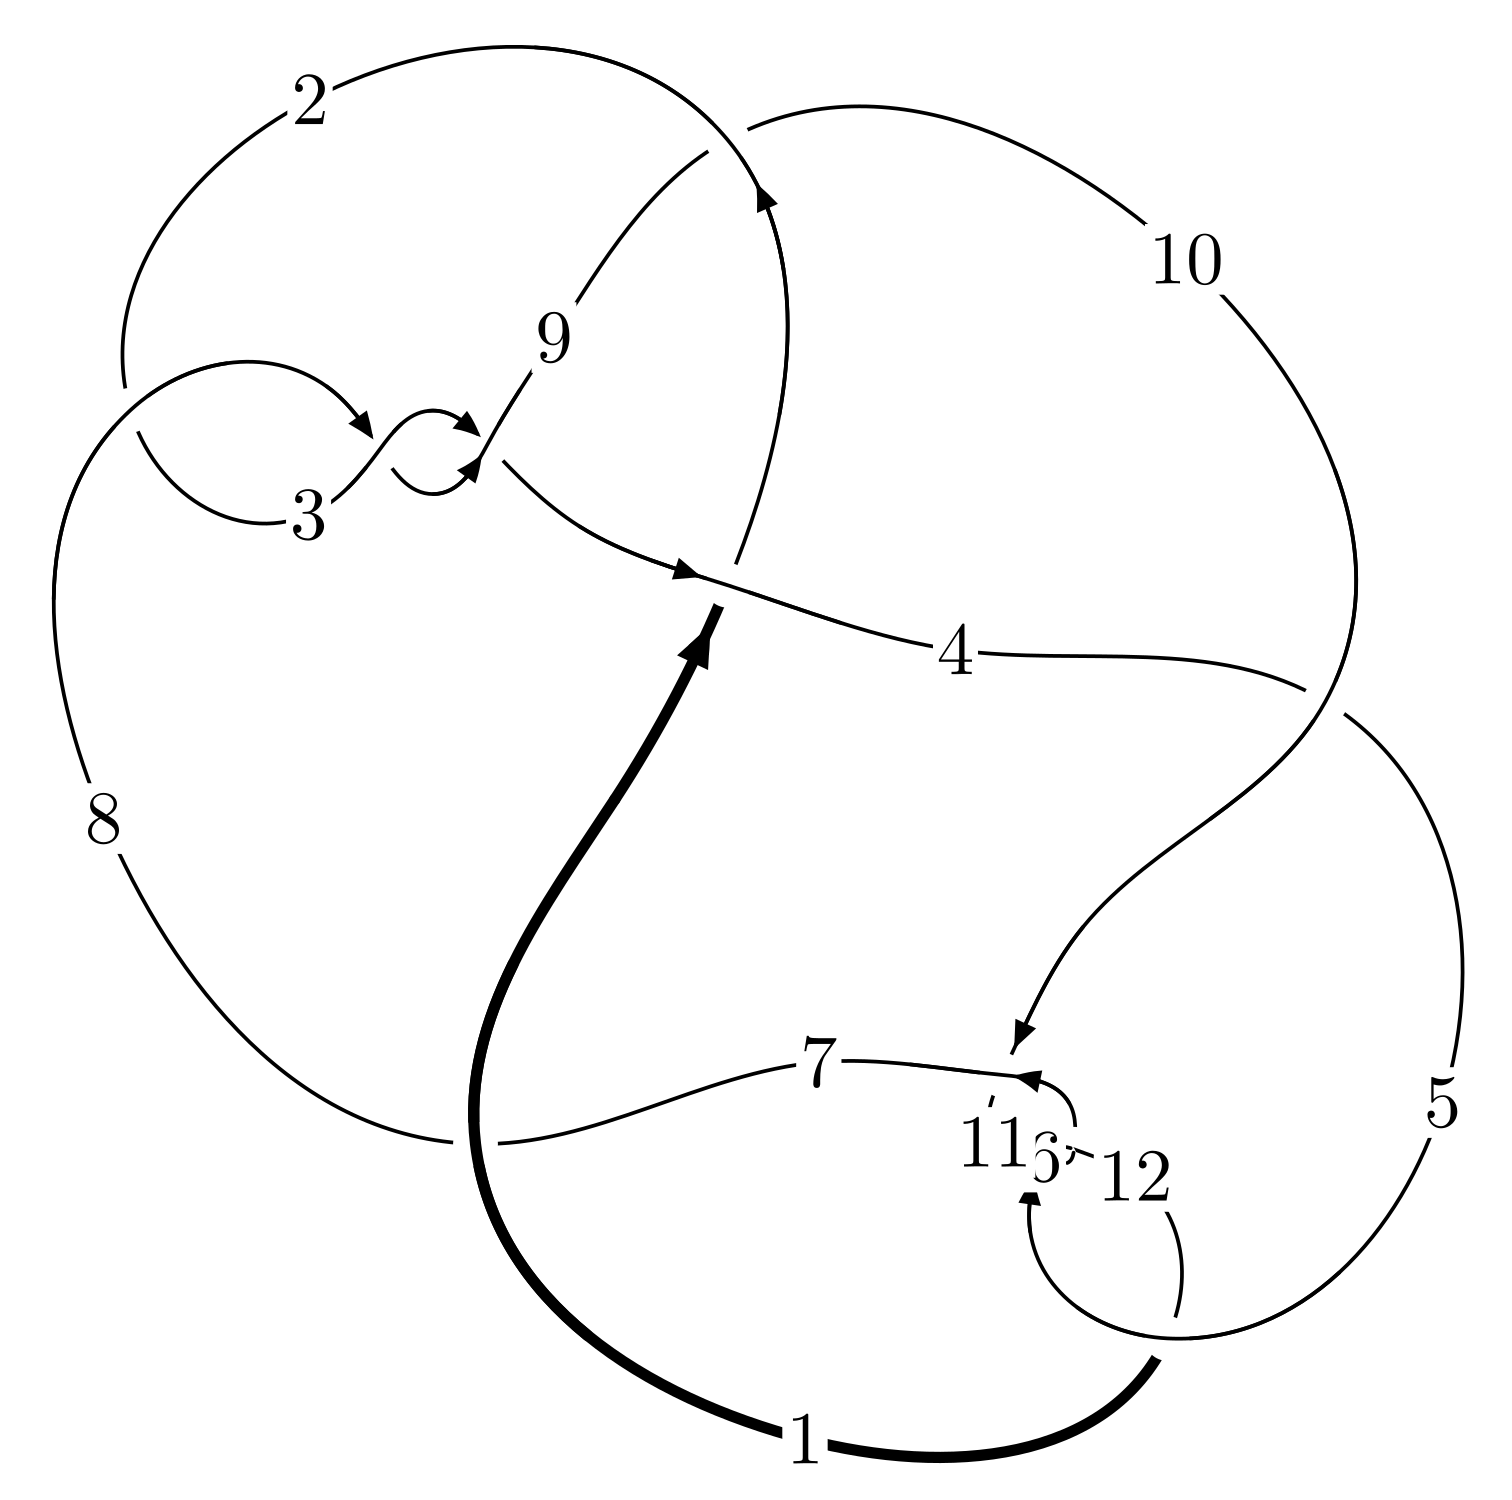
\includegraphics[width=112pt]{../../../GIT/diagram.site/Diagrams/png/1937_12a_1136.png}\\
\ \ \ A knot diagram\footnotemark}&
\allowdisplaybreaks
\textbf{Linearized knot diagam} \\
\cline{2-2}
 &
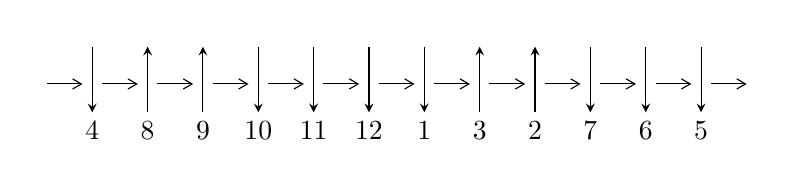
\begin{tikzpicture}[x=20pt, y=17pt]
	% nodes
	\node (C0) at (0, 0) {};
	\node (C1) at (1, 0) {};
	\node (C1U) at (1, +1) {};
	\node (C1D) at (1, -1) {4};

	\node (C2) at (2, 0) {};
	\node (C2U) at (2, +1) {};
	\node (C2D) at (2, -1) {8};

	\node (C3) at (3, 0) {};
	\node (C3U) at (3, +1) {};
	\node (C3D) at (3, -1) {9};

	\node (C4) at (4, 0) {};
	\node (C4U) at (4, +1) {};
	\node (C4D) at (4, -1) {10};

	\node (C5) at (5, 0) {};
	\node (C5U) at (5, +1) {};
	\node (C5D) at (5, -1) {11};

	\node (C6) at (6, 0) {};
	\node (C6U) at (6, +1) {};
	\node (C6D) at (6, -1) {12};

	\node (C7) at (7, 0) {};
	\node (C7U) at (7, +1) {};
	\node (C7D) at (7, -1) {1};

	\node (C8) at (8, 0) {};
	\node (C8U) at (8, +1) {};
	\node (C8D) at (8, -1) {3};

	\node (C9) at (9, 0) {};
	\node (C9U) at (9, +1) {};
	\node (C9D) at (9, -1) {2};

	\node (C10) at (10, 0) {};
	\node (C10U) at (10, +1) {};
	\node (C10D) at (10, -1) {7};

	\node (C11) at (11, 0) {};
	\node (C11U) at (11, +1) {};
	\node (C11D) at (11, -1) {6};

	\node (C12) at (12, 0) {};
	\node (C12U) at (12, +1) {};
	\node (C12D) at (12, -1) {5};
	\node (C13) at (13, 0) {};

	% arrows
	\draw[->,>={angle 60}]
	(C0) edge (C1) (C1) edge (C2) (C2) edge (C3) (C3) edge (C4) (C4) edge (C5) (C5) edge (C6) (C6) edge (C7) (C7) edge (C8) (C8) edge (C9) (C9) edge (C10) (C10) edge (C11) (C11) edge (C12) (C12) edge (C13) ;	\draw[->,>=stealth]
	(C1U) edge (C1D) (C2D) edge (C2U) (C3D) edge (C3U) (C4U) edge (C4D) (C5U) edge (C5D) (C6U) edge (C6D) (C7U) edge (C7D) (C8D) edge (C8U) (C9D) edge (C9U) (C10U) edge (C10D) (C11U) edge (C11D) (C12U) edge (C12D) ;
	\end{tikzpicture} \\
\hhline{~~} \\& 
\textbf{Solving Sequence} \\ \cline{2-2} 
 &
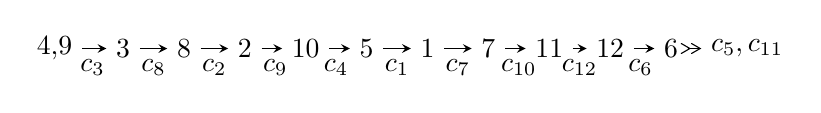
\begin{tikzpicture}[x=22pt, y=7pt]
	% node
	\node (A0) at (-1/8, 0) {4,9};
	\node (A1) at (1, 0) {3};
	\node (A2) at (2, 0) {8};
	\node (A3) at (3, 0) {2};
	\node (A4) at (4, 0) {10};
	\node (A5) at (5, 0) {5};
	\node (A6) at (6, 0) {1};
	\node (A7) at (7, 0) {7};
	\node (A8) at (8, 0) {11};
	\node (A9) at (9, 0) {12};
	\node (A10) at (10, 0) {6};
	\node (C1) at (1/2, -1) {$c_{3}$};
	\node (C2) at (3/2, -1) {$c_{8}$};
	\node (C3) at (5/2, -1) {$c_{2}$};
	\node (C4) at (7/2, -1) {$c_{9}$};
	\node (C5) at (9/2, -1) {$c_{4}$};
	\node (C6) at (11/2, -1) {$c_{1}$};
	\node (C7) at (13/2, -1) {$c_{7}$};
	\node (C8) at (15/2, -1) {$c_{10}$};
	\node (C9) at (17/2, -1) {$c_{12}$};
	\node (C10) at (19/2, -1) {$c_{6}$};
	\node (A11) at (45/4, 0) {$c_{5},c_{11}$};

	% edge
	\draw[->,>=stealth]	
	(A0) edge (A1) (A1) edge (A2) (A2) edge (A3) (A3) edge (A4) (A4) edge (A5) (A5) edge (A6) (A6) edge (A7) (A7) edge (A8) (A8) edge (A9) (A9) edge (A10) ;
	\draw[->>,>={angle 60}]	
	(A10) edge (A11);
\end{tikzpicture} \\ 

\end{tabular} \\

\footnotetext{
The image of knot diagram is generated by the software ``\textbf{Draw programme}" developed by Andrew Bartholomew(\url{http://www.layer8.co.uk/maths/draw/index.htm\#Running-draw}), where we modified some parts for our purpose(\url{https://github.com/CATsTAILs/LinksPainter}).
}\phantom \\ \newline 
\centering \textbf{Ideals for irreducible components\footnotemark of $X_{\text{par}}$} 
 
\begin{align*}
I^u_{1}&=\langle 
u^{66}+u^{65}+\cdots+2 u^2+1\rangle \\
I^u_{2}&=\langle 
u^6+u^5-2 u^4-2 u^3+1\rangle \\
I^u_{3}&=\langle 
u-1\rangle \\
\\
\end{align*}
\raggedright * 3 irreducible components of $\dim_{\mathbb{C}}=0$, with total 73 representations.\\
\footnotetext{All coefficients of polynomials are rational numbers. But the coefficients are sometimes approximated in decimal forms when there is not enough margin.}
\newpage
\renewcommand{\arraystretch}{1}
\centering \section*{I. $I^u_{1}= \langle u^{66}+u^{65}+\cdots+2 u^2+1 \rangle$}
\flushleft \textbf{(i) Arc colorings}\\
\begin{tabular}{m{7pt} m{180pt} m{7pt} m{180pt} }
\flushright $a_{4}=$&$\begin{pmatrix}1\\0\end{pmatrix}$ \\
\flushright $a_{9}=$&$\begin{pmatrix}0\\u\end{pmatrix}$ \\
\flushright $a_{3}=$&$\begin{pmatrix}1\\u^2\end{pmatrix}$ \\
\flushright $a_{8}=$&$\begin{pmatrix}- u\\- u^3+u\end{pmatrix}$ \\
\flushright $a_{2}=$&$\begin{pmatrix}- u^2+1\\- u^4+2 u^2\end{pmatrix}$ \\
\flushright $a_{10}=$&$\begin{pmatrix}u^5-2 u^3+u\\u^7-3 u^5+2 u^3+u\end{pmatrix}$ \\
\flushright $a_{5}=$&$\begin{pmatrix}u^{12}-5 u^{10}+9 u^8-6 u^6+u^2+1\\u^{14}-6 u^{12}+13 u^{10}-10 u^8-2 u^6+4 u^4+u^2\end{pmatrix}$ \\
\flushright $a_{1}=$&$\begin{pmatrix}- u^4+u^2+1\\- u^4+2 u^2\end{pmatrix}$ \\
\flushright $a_{7}=$&$\begin{pmatrix}- u^{11}+4 u^9-4 u^7-2 u^5+3 u^3\\- u^{11}+5 u^9-8 u^7+3 u^5+u^3+u\end{pmatrix}$ \\
\flushright $a_{11}=$&$\begin{pmatrix}- u^{29}+12 u^{27}+\cdots-2 u^3+u\\- u^{29}+13 u^{27}+\cdots+3 u^3+u\end{pmatrix}$ \\
\flushright $a_{12}=$&$\begin{pmatrix}u^{30}-13 u^{28}+\cdots+2 u^2+1\\u^{32}-14 u^{30}+\cdots-20 u^8+2 u^2\end{pmatrix}$ \\
\flushright $a_{6}=$&$\begin{pmatrix}u^{65}-28 u^{63}+\cdots+u+2\\u^{65}-29 u^{63}+\cdots+3 u^2+u\end{pmatrix}$\\&\end{tabular}
\flushleft \textbf{(ii) Obstruction class $= -1$}\\~\\
\flushleft \textbf{(iii) Cusp Shapes $= -4 u^{63}+116 u^{61}+\cdots+8 u-10$}\\~\\
\newpage\renewcommand{\arraystretch}{1}
\flushleft \textbf{(iv) u-Polynomials at the component}\newline \\
\begin{tabular}{m{50pt}|m{274pt}}
Crossings & \hspace{64pt}u-Polynomials at each crossing \\
\hline $$\begin{aligned}c_{1}\end{aligned}$$&$\begin{aligned}
&u^{66}-15 u^{65}+\cdots-1396 u+113
\end{aligned}$\\
\hline $$\begin{aligned}c_{2},c_{3},c_{8}\end{aligned}$$&$\begin{aligned}
&u^{66}- u^{65}+\cdots+2 u^2+1
\end{aligned}$\\
\hline $$\begin{aligned}c_{4},c_{7}\end{aligned}$$&$\begin{aligned}
&u^{66}-6 u^{65}+\cdots+84 u+8
\end{aligned}$\\
\hline $$\begin{aligned}c_{5},c_{6},c_{11}\end{aligned}$$&$\begin{aligned}
&u^{66}- u^{65}+\cdots+2 u^2+1
\end{aligned}$\\
\hline $$\begin{aligned}c_{9}\end{aligned}$$&$\begin{aligned}
&u^{66}+3 u^{65}+\cdots-6 u-1
\end{aligned}$\\
\hline $$\begin{aligned}c_{10},c_{12}\end{aligned}$$&$\begin{aligned}
&u^{66}+3 u^{65}+\cdots-2 u-1
\end{aligned}$\\
\hline
\end{tabular}\\~\\
\newpage\renewcommand{\arraystretch}{1}
\flushleft \textbf{(v) Riley Polynomials at the component}\newline \\
\begin{tabular}{m{50pt}|m{274pt}}
Crossings & \hspace{64pt}Riley Polynomials at each crossing \\
\hline $$\begin{aligned}c_{1}\end{aligned}$$&$\begin{aligned}
&y^{66}+13 y^{65}+\cdots+264176 y+12769
\end{aligned}$\\
\hline $$\begin{aligned}c_{2},c_{3},c_{8}\end{aligned}$$&$\begin{aligned}
&y^{66}-59 y^{65}+\cdots+4 y+1
\end{aligned}$\\
\hline $$\begin{aligned}c_{4},c_{7}\end{aligned}$$&$\begin{aligned}
&y^{66}-42 y^{65}+\cdots-8112 y+64
\end{aligned}$\\
\hline $$\begin{aligned}c_{5},c_{6},c_{11}\end{aligned}$$&$\begin{aligned}
&y^{66}-55 y^{65}+\cdots+4 y+1
\end{aligned}$\\
\hline $$\begin{aligned}c_{9}\end{aligned}$$&$\begin{aligned}
&y^{66}+y^{65}+\cdots-52 y+1
\end{aligned}$\\
\hline $$\begin{aligned}c_{10},c_{12}\end{aligned}$$&$\begin{aligned}
&y^{66}+37 y^{65}+\cdots-4 y+1
\end{aligned}$\\
\hline
\end{tabular}\\~\\
\newpage\flushleft \textbf{(vi) Complex Volumes and Cusp Shapes}
$$\begin{array}{c|c|c}  
\text{Solutions to }I^u_{1}& \I (\text{vol} + \sqrt{-1}CS) & \text{Cusp shape}\\
 \hline 
\begin{aligned}
u &= -0.990309 + 0.197371 I\end{aligned}
 & \phantom{-}0.77149 - 3.51641 I & -4.00000 + 4.68932 I \\ \hline\begin{aligned}
u &= -0.990309 - 0.197371 I\end{aligned}
 & \phantom{-}0.77149 + 3.51641 I & -4.00000 - 4.68932 I \\ \hline\begin{aligned}
u &= \phantom{-}0.983886 + 0.233964 I\end{aligned}
 & -4.05748 + 7.29975 I & \phantom{-0.000000 } 0. - 6.02392 I \\ \hline\begin{aligned}
u &= \phantom{-}0.983886 - 0.233964 I\end{aligned}
 & -4.05748 - 7.29975 I & \phantom{-0.000000 -}0. + 6.02392 I \\ \hline\begin{aligned}
u &= \phantom{-}0.917926\phantom{ +0.000000I}\end{aligned}
 & -1.63623\phantom{ +0.000000I} & -6.25380\phantom{ +0.000000I} \\ \hline\begin{aligned}
u &= -0.855417 + 0.248728 I\end{aligned}
 & -8.04962 + 0.09735 I & -10.00686 + 0.77062 I \\ \hline\begin{aligned}
u &= -0.855417 - 0.248728 I\end{aligned}
 & -8.04962 - 0.09735 I & -10.00686 - 0.77062 I \\ \hline\begin{aligned}
u &= \phantom{-}0.738976 + 0.315928 I\end{aligned}
 & -3.71204 - 7.38704 I & -6.03668 + 3.97983 I \\ \hline\begin{aligned}
u &= \phantom{-}0.738976 - 0.315928 I\end{aligned}
 & -3.71204 + 7.38704 I & -6.03668 - 3.97983 I \\ \hline\begin{aligned}
u &= \phantom{-}1.20059\phantom{ +0.000000I}\end{aligned}
 & -1.54443\phantom{ +0.000000I} & \phantom{-0.000000 } 0 \\ \hline\begin{aligned}
u &= \phantom{-}0.262184 + 0.729860 I\end{aligned}
 & -5.40381 + 11.28260 I & -8.66884 - 8.74113 I \\ \hline\begin{aligned}
u &= \phantom{-}0.262184 - 0.729860 I\end{aligned}
 & -5.40381 - 11.28260 I & -8.66884 + 8.74113 I \\ \hline\begin{aligned}
u &= -0.710255 + 0.292534 I\end{aligned}
 & \phantom{-}1.06112 + 3.49327 I & -1.18332 - 2.67462 I \\ \hline\begin{aligned}
u &= -0.710255 - 0.292534 I\end{aligned}
 & \phantom{-}1.06112 - 3.49327 I & -1.18332 + 2.67462 I \\ \hline\begin{aligned}
u &= -0.262033 + 0.720142 I\end{aligned}
 & -0.59286 - 7.29825 I & -4.05645 + 7.44817 I \\ \hline\begin{aligned}
u &= -0.262033 - 0.720142 I\end{aligned}
 & -0.59286 + 7.29825 I & -4.05645 - 7.44817 I \\ \hline\begin{aligned}
u &= -0.224274 + 0.729292 I\end{aligned}
 & -10.09160 - 3.88890 I & -12.88295 + 4.18648 I \\ \hline\begin{aligned}
u &= -0.224274 - 0.729292 I\end{aligned}
 & -10.09160 + 3.88890 I & -12.88295 - 4.18648 I \\ \hline\begin{aligned}
u &= \phantom{-}0.256468 + 0.700542 I\end{aligned}
 & -3.25124 + 3.34292 I & -7.24196 - 3.75335 I \\ \hline\begin{aligned}
u &= \phantom{-}0.256468 - 0.700542 I\end{aligned}
 & -3.25124 - 3.34292 I & -7.24196 + 3.75335 I \\ \hline\begin{aligned}
u &= \phantom{-}0.176621 + 0.719075 I\end{aligned}
 & -6.50527 - 3.62888 I & -10.79295 + 1.37881 I \\ \hline\begin{aligned}
u &= \phantom{-}0.176621 - 0.719075 I\end{aligned}
 & -6.50527 + 3.62888 I & -10.79295 - 1.37881 I \\ \hline\begin{aligned}
u &= \phantom{-}0.224321 + 0.695502 I\end{aligned}
 & -3.61835 + 3.40694 I & -9.07650 - 5.66068 I \\ \hline\begin{aligned}
u &= \phantom{-}0.224321 - 0.695502 I\end{aligned}
 & -3.61835 - 3.40694 I & -9.07650 + 5.66068 I \\ \hline\begin{aligned}
u &= -0.354761 + 0.564052 I\end{aligned}
 & \phantom{-}0.22062 - 5.60280 I & -3.25617 + 7.64930 I \\ \hline\begin{aligned}
u &= -0.354761 - 0.564052 I\end{aligned}
 & \phantom{-}0.22062 + 5.60280 I & -3.25617 - 7.64930 I \\ \hline\begin{aligned}
u &= -1.317080 + 0.220326 I\end{aligned}
 & -0.01372 - 5.66365 I & \phantom{-0.000000 } 0 \\ \hline\begin{aligned}
u &= -1.317080 - 0.220326 I\end{aligned}
 & -0.01372 + 5.66365 I & \phantom{-0.000000 } 0 \\ \hline\begin{aligned}
u &= \phantom{-}0.610474 + 0.243113 I\end{aligned}
 & -1.66667 + 0.22451 I & -3.98223 - 1.07282 I \\ \hline\begin{aligned}
u &= \phantom{-}0.610474 - 0.243113 I\end{aligned}
 & -1.66667 - 0.22451 I & -3.98223 + 1.07282 I\\
 \hline 
 \end{array}$$\newpage$$\begin{array}{c|c|c}  
\text{Solutions to }I^u_{1}& \I (\text{vol} + \sqrt{-1}CS) & \text{Cusp shape}\\
 \hline 
\begin{aligned}
u &= \phantom{-}0.368164 + 0.533247 I\end{aligned}
 & \phantom{-}4.23434 + 1.69125 I & \phantom{-}1.84273 - 4.33152 I \\ \hline\begin{aligned}
u &= \phantom{-}0.368164 - 0.533247 I\end{aligned}
 & \phantom{-}4.23434 - 1.69125 I & \phantom{-}1.84273 + 4.33152 I \\ \hline\begin{aligned}
u &= -1.354690 + 0.123144 I\end{aligned}
 & \phantom{-}3.75022 - 0.64597 I & \phantom{-0.000000 } 0 \\ \hline\begin{aligned}
u &= -1.354690 - 0.123144 I\end{aligned}
 & \phantom{-}3.75022 + 0.64597 I & \phantom{-0.000000 } 0 \\ \hline\begin{aligned}
u &= -0.392625 + 0.501531 I\end{aligned}
 & \phantom{-}0.44010 + 2.19041 I & -2.25026 + 0.38117 I \\ \hline\begin{aligned}
u &= -0.392625 - 0.501531 I\end{aligned}
 & \phantom{-}0.44010 - 2.19041 I & -2.25026 - 0.38117 I \\ \hline\begin{aligned}
u &= \phantom{-}1.355680 + 0.183514 I\end{aligned}
 & \phantom{-}4.57952 + 3.25192 I & \phantom{-0.000000 } 0 \\ \hline\begin{aligned}
u &= \phantom{-}1.355680 - 0.183514 I\end{aligned}
 & \phantom{-}4.57952 - 3.25192 I & \phantom{-0.000000 } 0 \\ \hline\begin{aligned}
u &= \phantom{-}0.102907 + 0.618996 I\end{aligned}
 & -4.43547 + 2.62457 I & -11.91060 - 4.28004 I \\ \hline\begin{aligned}
u &= \phantom{-}0.102907 - 0.618996 I\end{aligned}
 & -4.43547 - 2.62457 I & -11.91060 + 4.28004 I \\ \hline\begin{aligned}
u &= \phantom{-}1.367250 + 0.272605 I\end{aligned}
 & \phantom{-}3.25888 + 3.51289 I & \phantom{-0.000000 } 0 \\ \hline\begin{aligned}
u &= \phantom{-}1.367250 - 0.272605 I\end{aligned}
 & \phantom{-}3.25888 - 3.51289 I & \phantom{-0.000000 } 0 \\ \hline\begin{aligned}
u &= -1.408740 + 0.110369 I\end{aligned}
 & \phantom{-}4.37917 - 1.51275 I & \phantom{-0.000000 } 0 \\ \hline\begin{aligned}
u &= -1.408740 - 0.110369 I\end{aligned}
 & \phantom{-}4.37917 + 1.51275 I & \phantom{-0.000000 } 0 \\ \hline\begin{aligned}
u &= -1.38787 + 0.27581 I\end{aligned}
 & \phantom{-}1.50869 - 6.93616 I & \phantom{-0.000000 } 0 \\ \hline\begin{aligned}
u &= -1.38787 - 0.27581 I\end{aligned}
 & \phantom{-}1.50869 + 6.93616 I & \phantom{-0.000000 } 0 \\ \hline\begin{aligned}
u &= \phantom{-}1.41479 + 0.09089 I\end{aligned}
 & \phantom{-}7.41801 - 2.39956 I & \phantom{-0.000000 } 0 \\ \hline\begin{aligned}
u &= \phantom{-}1.41479 - 0.09089 I\end{aligned}
 & \phantom{-}7.41801 + 2.39956 I & \phantom{-0.000000 } 0 \\ \hline\begin{aligned}
u &= \phantom{-}1.38826 + 0.29191 I\end{aligned}
 & -4.97005 + 7.59047 I & \phantom{-0.000000 } 0 \\ \hline\begin{aligned}
u &= \phantom{-}1.38826 - 0.29191 I\end{aligned}
 & -4.97005 - 7.59047 I & \phantom{-0.000000 } 0 \\ \hline\begin{aligned}
u &= -1.42024 + 0.07916 I\end{aligned}
 & \phantom{-}2.81245 + 6.36681 I & \phantom{-0.000000 } 0 \\ \hline\begin{aligned}
u &= -1.42024 - 0.07916 I\end{aligned}
 & \phantom{-}2.81245 - 6.36681 I & \phantom{-0.000000 } 0 \\ \hline\begin{aligned}
u &= -1.40307 + 0.27814 I\end{aligned}
 & \phantom{-}2.03846 - 6.90566 I & \phantom{-0.000000 } 0 \\ \hline\begin{aligned}
u &= -1.40307 - 0.27814 I\end{aligned}
 & \phantom{-}2.03846 + 6.90566 I & \phantom{-0.000000 } 0 \\ \hline\begin{aligned}
u &= \phantom{-}1.42052 + 0.19384 I\end{aligned}
 & \phantom{-}6.18270 + 0.37995 I & \phantom{-0.000000 } 0 \\ \hline\begin{aligned}
u &= \phantom{-}1.42052 - 0.19384 I\end{aligned}
 & \phantom{-}6.18270 - 0.37995 I & \phantom{-0.000000 } 0 \\ \hline\begin{aligned}
u &= -1.42012 + 0.20531 I\end{aligned}
 & \phantom{-}9.92026 - 4.41693 I & \phantom{-0.000000 } 0 \\ \hline\begin{aligned}
u &= -1.42012 - 0.20531 I\end{aligned}
 & \phantom{-}9.92026 + 4.41693 I & \phantom{-0.000000 } 0 \\ \hline\begin{aligned}
u &= \phantom{-}1.40654 + 0.28588 I\end{aligned}
 & \phantom{-}4.72530 + 10.95400 I & \phantom{-0.000000 } 0 \\ \hline\begin{aligned}
u &= \phantom{-}1.40654 - 0.28588 I\end{aligned}
 & \phantom{-}4.72530 - 10.95400 I & \phantom{-0.000000 } 0\\
 \hline 
 \end{array}$$\newpage$$\begin{array}{c|c|c}  
\text{Solutions to }I^u_{1}& \I (\text{vol} + \sqrt{-1}CS) & \text{Cusp shape}\\
 \hline 
\begin{aligned}
u &= \phantom{-}1.42058 + 0.21544 I\end{aligned}
 & \phantom{-}5.87848 + 8.46734 I & \phantom{-0.000000 } 0 \\ \hline\begin{aligned}
u &= \phantom{-}1.42058 - 0.21544 I\end{aligned}
 & \phantom{-}5.87848 - 8.46734 I & \phantom{-0.000000 } 0 \\ \hline\begin{aligned}
u &= -1.40733 + 0.29033 I\end{aligned}
 & -0.0836 - 14.9873 I & \phantom{-0.000000 } 0 \\ \hline\begin{aligned}
u &= -1.40733 - 0.29033 I\end{aligned}
 & -0.0836 + 14.9873 I & \phantom{-0.000000 } 0 \\ \hline\begin{aligned}
u &= -0.148067 + 0.449066 I\end{aligned}
 & -0.202946 - 0.853104 I & -4.89270 + 7.93904 I \\ \hline\begin{aligned}
u &= -0.148067 - 0.449066 I\end{aligned}
 & -0.202946 + 0.853104 I & -4.89270 - 7.93904 I\\
 \hline 
 \end{array}$$\newpage\newpage\renewcommand{\arraystretch}{1}
\centering \section*{II. $I^u_{2}= \langle u^6+u^5-2 u^4-2 u^3+1 \rangle$}
\flushleft \textbf{(i) Arc colorings}\\
\begin{tabular}{m{7pt} m{180pt} m{7pt} m{180pt} }
\flushright $a_{4}=$&$\begin{pmatrix}1\\0\end{pmatrix}$ \\
\flushright $a_{9}=$&$\begin{pmatrix}0\\u\end{pmatrix}$ \\
\flushright $a_{3}=$&$\begin{pmatrix}1\\u^2\end{pmatrix}$ \\
\flushright $a_{8}=$&$\begin{pmatrix}- u\\- u^3+u\end{pmatrix}$ \\
\flushright $a_{2}=$&$\begin{pmatrix}- u^2+1\\- u^4+2 u^2\end{pmatrix}$ \\
\flushright $a_{10}=$&$\begin{pmatrix}u^5-2 u^3+u\\1\end{pmatrix}$ \\
\flushright $a_{5}=$&$\begin{pmatrix}u^5-2 u^3+u+1\\1\end{pmatrix}$ \\
\flushright $a_{1}=$&$\begin{pmatrix}- u^4+u^2+1\\- u^4+2 u^2\end{pmatrix}$ \\
\flushright $a_{7}=$&$\begin{pmatrix}- u^4+u^2- u+1\\- u^4- u^3+2 u^2+u\end{pmatrix}$ \\
\flushright $a_{11}=$&$\begin{pmatrix}- u^4+u^2+u-1\\u^5-2 u^3- u^2+u+1\end{pmatrix}$ \\
\flushright $a_{12}=$&$\begin{pmatrix}u^3- u^2+1\\- u^4+u^3+2 u^2- u\end{pmatrix}$ \\
\flushright $a_{6}=$&$\begin{pmatrix}- u^3+u^2+1\\- u^5+u^3+u^2+u\end{pmatrix}$\\&\end{tabular}
\flushleft \textbf{(ii) Obstruction class $= -1$}\\~\\
\flushleft \textbf{(iii) Cusp Shapes $= -6$}\\~\\
\newpage\renewcommand{\arraystretch}{1}
\flushleft \textbf{(iv) u-Polynomials at the component}\newline \\
\begin{tabular}{m{50pt}|m{274pt}}
Crossings & \hspace{64pt}u-Polynomials at each crossing \\
\hline $$\begin{aligned}c_{1}\end{aligned}$$&$\begin{aligned}
&u^6- u^5+2 u^3+2 u^2-4 u+1
\end{aligned}$\\
\hline $$\begin{aligned}c_{2},c_{3},c_{5}\\c_{6},c_{8},c_{11}\end{aligned}$$&$\begin{aligned}
&u^6- u^5-2 u^4+2 u^3+1
\end{aligned}$\\
\hline $$\begin{aligned}c_{4},c_{7}\end{aligned}$$&$\begin{aligned}
&(u+1)^6
\end{aligned}$\\
\hline $$\begin{aligned}c_{9},c_{10},c_{12}\end{aligned}$$&$\begin{aligned}
&u^6+u^4-2 u^3+2 u^2-2 u-1
\end{aligned}$\\
\hline
\end{tabular}\\~\\
\newpage\renewcommand{\arraystretch}{1}
\flushleft \textbf{(v) Riley Polynomials at the component}\newline \\
\begin{tabular}{m{50pt}|m{274pt}}
Crossings & \hspace{64pt}Riley Polynomials at each crossing \\
\hline $$\begin{aligned}c_{1}\end{aligned}$$&$\begin{aligned}
&y^6- y^5+8 y^4-10 y^3+20 y^2-12 y+1
\end{aligned}$\\
\hline $$\begin{aligned}c_{2},c_{3},c_{5}\\c_{6},c_{8},c_{11}\end{aligned}$$&$\begin{aligned}
&y^6-5 y^5+8 y^4-2 y^3-4 y^2+1
\end{aligned}$\\
\hline $$\begin{aligned}c_{4},c_{7}\end{aligned}$$&$\begin{aligned}
&(y-1)^6
\end{aligned}$\\
\hline $$\begin{aligned}c_{9},c_{10},c_{12}\end{aligned}$$&$\begin{aligned}
&y^6+2 y^5+5 y^4-2 y^3-6 y^2-8 y+1
\end{aligned}$\\
\hline
\end{tabular}\\~\\
\newpage\flushleft \textbf{(vi) Complex Volumes and Cusp Shapes}
$$\begin{array}{c|c|c}  
\text{Solutions to }I^u_{2}& \I (\text{vol} + \sqrt{-1}CS) & \text{Cusp shape}\\
 \hline 
\begin{aligned}
u &= \phantom{-}0.733459\phantom{ +0.000000I}\end{aligned}
 & -1.64493\phantom{ +0.000000I} & -6.00000\phantom{ +0.000000I} \\ \hline\begin{aligned}
u &= -0.181278 + 0.698849 I\end{aligned}
 & -1.64493\phantom{ +0.000000I} & -6.00000\phantom{ +0.000000I} \\ \hline\begin{aligned}
u &= -0.181278 - 0.698849 I\end{aligned}
 & -1.64493\phantom{ +0.000000I} & -6.00000\phantom{ +0.000000I} \\ \hline\begin{aligned}
u &= \phantom{-}1.35202\phantom{ +0.000000I}\end{aligned}
 & -1.64493\phantom{ +0.000000I} & -6.00000\phantom{ +0.000000I} \\ \hline\begin{aligned}
u &= -1.361460 + 0.284643 I\end{aligned}
 & -1.64493\phantom{ +0.000000I} & -6.00000\phantom{ +0.000000I} \\ \hline\begin{aligned}
u &= -1.361460 - 0.284643 I\end{aligned}
 & -1.64493\phantom{ +0.000000I} & -6.00000\phantom{ +0.000000I}\\
 \hline 
 \end{array}$$\newpage\newpage\renewcommand{\arraystretch}{1}
\centering \section*{III. $I^u_{3}= \langle u-1 \rangle$}
\flushleft \textbf{(i) Arc colorings}\\
\begin{tabular}{m{7pt} m{180pt} m{7pt} m{180pt} }
\flushright $a_{4}=$&$\begin{pmatrix}1\\0\end{pmatrix}$ \\
\flushright $a_{9}=$&$\begin{pmatrix}0\\1\end{pmatrix}$ \\
\flushright $a_{3}=$&$\begin{pmatrix}1\\1\end{pmatrix}$ \\
\flushright $a_{8}=$&$\begin{pmatrix}-1\\0\end{pmatrix}$ \\
\flushright $a_{2}=$&$\begin{pmatrix}0\\1\end{pmatrix}$ \\
\flushright $a_{10}=$&$\begin{pmatrix}0\\1\end{pmatrix}$ \\
\flushright $a_{5}=$&$\begin{pmatrix}1\\1\end{pmatrix}$ \\
\flushright $a_{1}=$&$\begin{pmatrix}1\\1\end{pmatrix}$ \\
\flushright $a_{7}=$&$\begin{pmatrix}0\\1\end{pmatrix}$ \\
\flushright $a_{11}=$&$\begin{pmatrix}0\\1\end{pmatrix}$ \\
\flushright $a_{12}=$&$\begin{pmatrix}1\\1\end{pmatrix}$ \\
\flushright $a_{6}=$&$\begin{pmatrix}1\\2\end{pmatrix}$\\&\end{tabular}
\flushleft \textbf{(ii) Obstruction class $= -1$}\\~\\
\flushleft \textbf{(iii) Cusp Shapes $= -6$}\\~\\
\newpage\renewcommand{\arraystretch}{1}
\flushleft \textbf{(iv) u-Polynomials at the component}\newline \\
\begin{tabular}{m{50pt}|m{274pt}}
Crossings & \hspace{64pt}u-Polynomials at each crossing \\
\hline $$\begin{aligned}c_{1}\end{aligned}$$&$\begin{aligned}
&u-1
\end{aligned}$\\
\hline $$\begin{aligned}c_{2},c_{3},c_{4}\\c_{5},c_{6},c_{7}\\c_{8},c_{11}\end{aligned}$$&$\begin{aligned}
&u+1
\end{aligned}$\\
\hline $$\begin{aligned}c_{9},c_{10},c_{12}\end{aligned}$$&$\begin{aligned}
&u
\end{aligned}$\\
\hline
\end{tabular}\\~\\
\newpage\renewcommand{\arraystretch}{1}
\flushleft \textbf{(v) Riley Polynomials at the component}\newline \\
\begin{tabular}{m{50pt}|m{274pt}}
Crossings & \hspace{64pt}Riley Polynomials at each crossing \\
\hline $$\begin{aligned}c_{1},c_{2},c_{3}\\c_{4},c_{5},c_{6}\\c_{7},c_{8},c_{11}\end{aligned}$$&$\begin{aligned}
&y-1
\end{aligned}$\\
\hline $$\begin{aligned}c_{9},c_{10},c_{12}\end{aligned}$$&$\begin{aligned}
&y
\end{aligned}$\\
\hline
\end{tabular}\\~\\
\newpage\flushleft \textbf{(vi) Complex Volumes and Cusp Shapes}
$$\begin{array}{c|c|c}  
\text{Solutions to }I^u_{3}& \I (\text{vol} + \sqrt{-1}CS) & \text{Cusp shape}\\
 \hline 
\begin{aligned}
u &= \phantom{-}1.00000\phantom{ +0.000000I}\end{aligned}
 & -1.64493\phantom{ +0.000000I} & -6.00000\phantom{ +0.000000I}\\
 \hline 
 \end{array}$$\newpage
\newpage\renewcommand{\arraystretch}{1}
\centering \section*{ IV. u-Polynomials}
\begin{tabular}{m{50pt}|m{274pt}}
Crossings & \hspace{64pt}u-Polynomials at each crossing \\
\hline $$\begin{aligned}c_{1}\end{aligned}$$&$\begin{aligned}
&(u-1)(u^6- u^5+\cdots-4 u+1)(u^{66}-15 u^{65}+\cdots-1396 u+113)
\end{aligned}$\\
\hline $$\begin{aligned}c_{2},c_{3},c_{8}\end{aligned}$$&$\begin{aligned}
&(u+1)(u^6- u^5-2 u^4+2 u^3+1)(u^{66}- u^{65}+\cdots+2 u^2+1)
\end{aligned}$\\
\hline $$\begin{aligned}c_{4},c_{7}\end{aligned}$$&$\begin{aligned}
&((u+1)^7)(u^{66}-6 u^{65}+\cdots+84 u+8)
\end{aligned}$\\
\hline $$\begin{aligned}c_{5},c_{6},c_{11}\end{aligned}$$&$\begin{aligned}
&(u+1)(u^6- u^5-2 u^4+2 u^3+1)(u^{66}- u^{65}+\cdots+2 u^2+1)
\end{aligned}$\\
\hline $$\begin{aligned}c_{9}\end{aligned}$$&$\begin{aligned}
&u(u^6+u^4+\cdots-2 u-1)(u^{66}+3 u^{65}+\cdots-6 u-1)
\end{aligned}$\\
\hline $$\begin{aligned}c_{10},c_{12}\end{aligned}$$&$\begin{aligned}
&u(u^6+u^4+\cdots-2 u-1)(u^{66}+3 u^{65}+\cdots-2 u-1)
\end{aligned}$\\
\hline
\end{tabular}\newpage\renewcommand{\arraystretch}{1}
\centering \section*{ V. Riley Polynomials}
\begin{tabular}{m{50pt}|m{274pt}}
Crossings & \hspace{64pt}Riley Polynomials at each crossing \\
\hline $$\begin{aligned}c_{1}\end{aligned}$$&$\begin{aligned}
&(y-1)(y^6- y^5+8 y^4-10 y^3+20 y^2-12 y+1)\\
&\cdot(y^{66}+13 y^{65}+\cdots+264176 y+12769)
\end{aligned}$\\
\hline $$\begin{aligned}c_{2},c_{3},c_{8}\end{aligned}$$&$\begin{aligned}
&(y-1)(y^6-5 y^5+\cdots-4 y^2+1)(y^{66}-59 y^{65}+\cdots+4 y+1)
\end{aligned}$\\
\hline $$\begin{aligned}c_{4},c_{7}\end{aligned}$$&$\begin{aligned}
&((y-1)^7)(y^{66}-42 y^{65}+\cdots-8112 y+64)
\end{aligned}$\\
\hline $$\begin{aligned}c_{5},c_{6},c_{11}\end{aligned}$$&$\begin{aligned}
&(y-1)(y^6-5 y^5+\cdots-4 y^2+1)(y^{66}-55 y^{65}+\cdots+4 y+1)
\end{aligned}$\\
\hline $$\begin{aligned}c_{9}\end{aligned}$$&$\begin{aligned}
&y(y^6+2 y^5+\cdots-8 y+1)(y^{66}+y^{65}+\cdots-52 y+1)
\end{aligned}$\\
\hline $$\begin{aligned}c_{10},c_{12}\end{aligned}$$&$\begin{aligned}
&y(y^6+2 y^5+\cdots-8 y+1)(y^{66}+37 y^{65}+\cdots-4 y+1)
\end{aligned}$\\
\hline
\end{tabular}
\vskip 2pc
\end{document}